\chptr{Relatività del Moto}
\marginpar{\minitoc}

\epigraph{\emph{``That view of things would be normal for me if I normally walked on my hands.''}}{\href{https://www.youtube.com/watch?v=bJMYoj4hHqU}{\textcolor{blue}{\textit{Frames of Reference (1960) - Hume, Ivey}}}}

Cominciamo questo capitolo ponendo al lettore una domanda:

\begin{center}
    \textit{Sei aristotelica/o oppure copernicana/o?}
\end{center}

\noindent Senza soffermarci troppo su cosa essa intenda,
sottolineamo brevemente che ciò di cui si tratta in questo capitolo
è stato uno dei temi più controversi nella storia della fisica, quello
che forse ha sconvolto di più convinzioni un tempo ben radicate e
che ha infiammato dibattiti che hanno pure fatto la storia della
letteratura\footnote{\href{https://youtu.be/0kxarmulkiA?feature=shared&t=6180}{\textcolor{blue}{\textit{Marco Paolini - ITIS Galileo}}} (circa 10 minuti a partire dal tempo 1:43:00).}. E non è tutto qui: Gli ultimi grandi sviluppi della relatività
del moto sono avvenuti poco più di un secolo fa ad opera di Einstein
e molti altri e i cambiamenti da loro apportati hanno condotto a
stravolgimenti ancora più bizzarri. Perché ciò che questo ramo della
fisica rivela è che più osserviamo con attenzione la realtà, più essa non
è come un attimo prima poteva sembrare. Per tale motivo la relatività può
essere allo stesso tempo semplice e complessa, perché offre una visione
del tutto insolita di ciò che ci appare come ``normale''.


\section{Sistemi di riferimento}
``Relativo'' è un termine che ben si sposa con l'espressione ``a qualcosa''.
Quel qualcosa viene definito nelle teorie relativistiche della fisica
\textit{sistema di riferimento}, che intuitivamente rappresenta il punto di
vista dal quale si effettuano delle misurazioni o semplici osservazioni di
fenomeni. Ricordiamo che tra le coordinate di un sistema di riferimento
è presente anche il tempo.

\begin{tcolorbox}[colback = yellow!30, colframe = yellow!30!black, title = {Sistema di riferimento}]
    Un insieme di strumenti geometrico-algebrici, di coordinate solidali con un
    oggetto arbitrario, e di procedure che consentono di individuare la posizione
    di un punto di uno spazio metrico.
\end{tcolorbox}

Una volta fissato il sistema di riferimento, tutte le misurazioni devono
essere coerenti con esso, se si intende adottare quel punto di vista.
Quando diciamo che un'auto viaggia a 110 km/h, stiamo in realtà fornendo
un'informazione incompleta, perché sottintendiamo che tale misurazione
sia stata effettuata rispetto alla strada. Non potremmo dire la stessa
cosa se viaggiassimo su un'altra auto che affianca la prima, con stessa
direzione e verso: Diremmo che
l'auto che prima, vista dalla strada, si muoveva a 110 km/h ora sta viaggiando con velocità
minore rispetto a noi. Il moto di un corpo è sempre relativo a un sistema di riferimento.
Cambiando il sistema, il moto cambia. Vedremo nei prossimi paragrafi
che però non tutti i sistemi di riferimento sono uguali e possono
distinguersi in \textit{inerziali} e \textit{non inerziali}.

Il cambiamento riguarda anche le traiettorie: Se lanciassimo una pallina
verso l'alto mentre viaggiamo sulla carrozza di un treno con velocità
costante, vedremmo la pallina salire e scendere su una linea retta.
Un osservatore esterno, invece vedrebbe la pallina muoversi secondo
una traiettoria parabolica. Vedremo che i moti si compongono
ed è necessario effettuare trasformazioni tra le coordinate dei
sistemi di riferimento.

\section{Trasformazioni tra sistemi di riferimento}
Lorem ipsum dolor sit amet.

\begin{marginfigure}
    \centering
    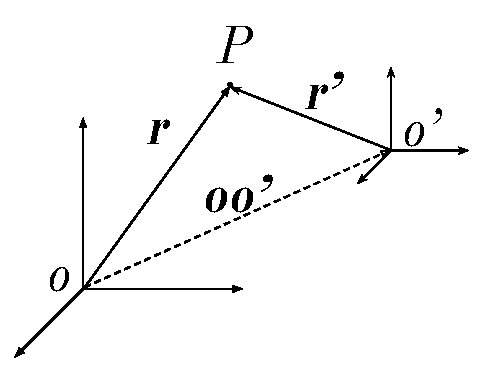
\includegraphics[width = \marginparwidth]{sistemirelativi.pdf}
    \caption{Relazione tra due sistemi di riferimento che misurano
    la posizione del punto $P$.}
\end{marginfigure}


\section{Principio di relatività galileiana}

\begin{tcolorbox}[colback = yellow!30, colframe = yellow!30!black, title = {Principio dei relatività galileiana}]
Le leggi della dinamica newtoniana hanno la stessa forma in tutti i
sistemi di riferimento inerziali.

Con riferimento alle proprietà cinematiche di posizione e velocità di
un punto materiale, il legame tra un sistema di riferimento inerziale,
con origine $o$, e un altro sistema di riferimento inerziale, con
origine $o'$, è descritta dalla seguente trasformazione:

\begin{align}
\begin{cases}
    \vecsymb{r} = \vecsymb{r}' + \vecsymb{oo}'\\
    \vecsymb{v} = \vecsymb{v}' + \vecsymb{v}_{o'}
\end{cases}
\end{align}
\end{tcolorbox}


\section{Forze apparenti}


\subsection{L'ascensore}

%\section{Approfondimento: RR}
%Questa sezione è interamente dedicata alla relatività ristretta, sviluppata
%nelle sue forme più celebri da Einstein nei primi lustri del Ventesimo secolo.
%Vogliamo dare un assaggio di questa teoria per vari motivi: Si tratta in primo
%luogo di fisica classica (gli strumenti matematici impiegati sono pressoché gli stessi); essa è inoltre un buon esempio di ridefinizione e affinamento
%radicali di teorie precedenti, innanzitutto la relatività galileiana, e convinzioni
%comuni.

%\subsection{I principi della relatività ristretta}